\documentclass[12pt]{article}

% Packages
\usepackage{amsmath, amssymb, mathtools}
\usepackage{graphicx}
\usepackage{physics}
\usepackage{geometry}
\usepackage{enumitem}
\usepackage{bm}
\usepackage{listings}
\usepackage{xcolor}
\usepackage{float}

% Geometry settings
\geometry{letterpaper, margin=1in}
\setlength{\parindent}{0pt}

\definecolor{codegreen}{rgb}{0,0.6,0}
\definecolor{codegray}{rgb}{0.5,0.5,0.5}
\definecolor{codepurple}{rgb}{0.58,0,0.82}
\definecolor{backcolour}{rgb}{0.95,0.95,0.92}

\lstdefinestyle{mystyle}{
    backgroundcolor=\color{backcolour},   
    commentstyle=\color{codegreen},
    keywordstyle=\color{magenta},
    numberstyle=\tiny\color{codegray},
    stringstyle=\color{codepurple},
    basicstyle=\ttfamily\footnotesize,
    breakatwhitespace=false,         
    breaklines=true,                 
    captionpos=b,                    
    keepspaces=true,                 
    numbers=left,                    
    numbersep=5pt,                  
    showspaces=false,                
    showstringspaces=false,
    showtabs=false,                  
    tabsize=2
}

\lstset{style=mystyle}

% Title
\title{ECE 148 Homework 6}
\author{Sanjot Bains}
\date{\today}

\begin{document}

\maketitle

\section*{I. Interpolation by DFT}
Consider a real periodic signal $f(t)$ of period $T$. The signal has 7 harmonics, for $m = 1, 2, 3, \ldots, 7$:
\[ f(t) = \sum_{m=1}^7 a_m \sin(m \omega_0 t) \]
where $\omega_0 = \frac{2\pi}{T}$ and the 7 coefficients $\{a_m\}$ are formed with the 7-digit perm number: 9587189.

\begin{lstlisting}[language=Octave, caption=Signal Definition]
T = 1; % Period of the signal
w_0 = 2 * pi / T; % Fundamental frequency
a_m = [9 5 8 7 1 8 9]; % Amplitude of harmonics

f = @(t) a_m(1) * sin(1 * w_0 * t) + a_m(2) * sin(2 * w_0 * t) + ...
         a_m(3) * sin(3 * w_0 * t) + a_m(4) * sin(4 * w_0 * t) + ...
         a_m(5) * sin(5 * w_0 * t) + a_m(6) * sin(6 * w_0 * t) + ...
         a_m(7) * sin(7 * w_0 * t);
\end{lstlisting}

We take 16 uniform samples within one period with sample spacing $\Delta t = \frac{T}{16}$ to form a short 16-point sequence $\{f(n)\}$, where $n = 0, 1, 2, \ldots, 15$.

\begin{lstlisting}[language=Octave, caption=Sampling]
delta_T = T / 16; % Sampling interval
t_samples = 0:delta_T:(T-delta_T); % Sampled time vector
f_n = f(t_samples); % Sampled function values {f(n = 0, 1, ... , 15)}
\end{lstlisting}

Subsequently, we take a 16-point DFT of the sequence to obtain the 16-point spectral sequence F(k), where k = 0, 1, 2, ... , 15.
\[  F(k) = DFT_{N = 16} \{f(n)\}  \]

\begin{lstlisting}[language=Octave, caption=16-pt DFT]
F_k = fft(f_n); % F(k) = DFT of f(n = 0, 1, ... , 15)
F_k_shifted = fftshift(F_k);
\end{lstlisting}


\newpage
\subsection*{1. Interpolation of the DFT Spectrum}
The sequence $f(n)$ is extended to 64 points by padding 48 zeros. The extended sequence $f_a(n)$ is in the form:
\[ f_a(n) = \begin{cases}
f(n) & n = 0, 1, 2, \ldots, 15 \\
0 & n = 16, 17, 18, \ldots, 63
\end{cases} \]

\begin{lstlisting}[language=Octave, caption=Zero-Padded Time Sequence]
f_a = zeros(1, 64);
f_a(1:16) = f_n;
\end{lstlisting}

\vspace{0.5 cm}
We then compute the DFT of the 64-pt sequence:
\[ F_a(k) = DFT_{N = 64} \{f_a(n)\} \]

\begin{lstlisting}[language=Octave, caption=DFT of 64-pt Sequence]
F_a_shifted = fftshift(fft(f_a));
\end{lstlisting}

\begin{figure}[H]
    \centering
    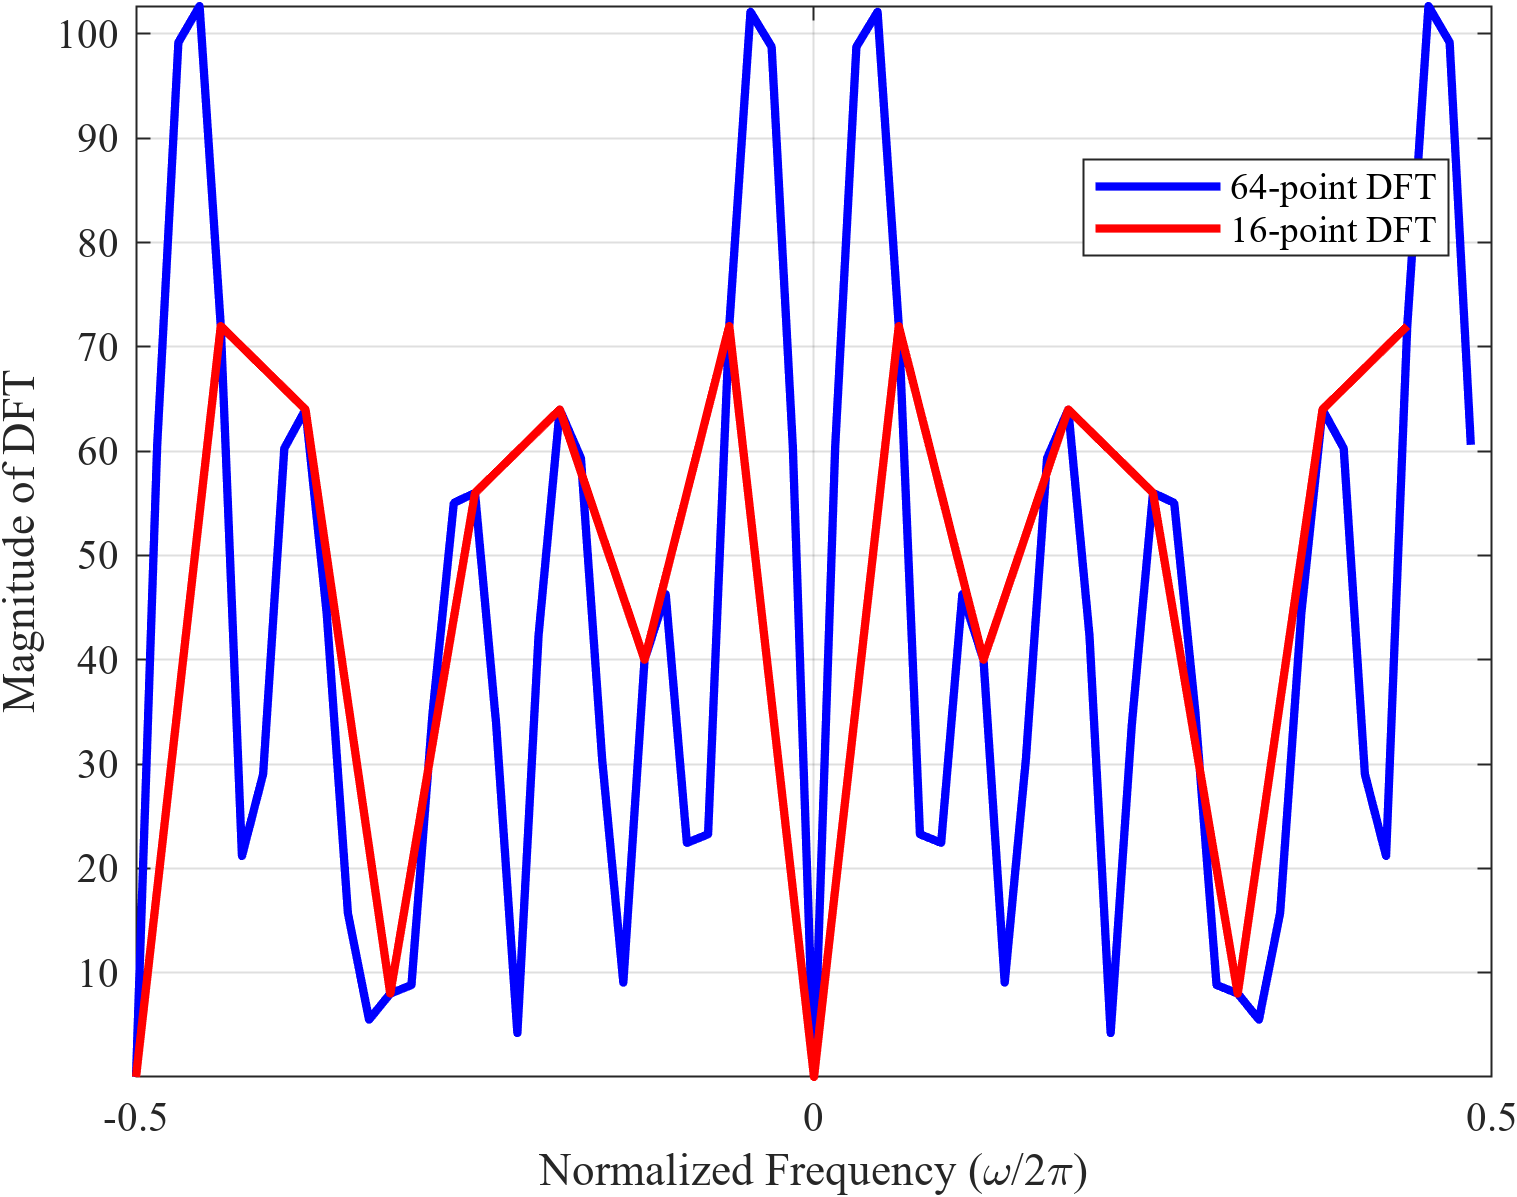
\includegraphics[width=0.8\textwidth]{F_a.png}
    \caption{Comparison of 64-point and 16-point DFT}
\end{figure}

$F_a(k)$ seems to contain more information than $F(k)$, a more granular view of the component frequencies. I had to rescale the frequency axis to overlap the 64-pt and 16-pt sequences. The two plots are identical at every 4th point, where the 16-pt sequence is defined.

\newpage
\subsection*{2. Interpolation in Time Domain}
The 16-point spectral sequence $F(k)$ is extended to 64 points by inserting 48 zeros in the middle. 

\begin{lstlisting}[language=Octave, caption=Zero-Padded Frequency Sequence]
F_b = zeros(1, 64);
F_b(1:8) = F_k(1:8);
F_b(57:64) = F_k(9:16);
F_b = 4 * F_b;
\end{lstlisting}

\vspace{0.5 cm}
The resulting interpolated time-domain signal $f_b(n)$ is computed using IDFT:
\[  f_b(n) = IDFT_{N = 64} \{F_b(k)\} \]

\begin{lstlisting}[language=Octave, caption=IFFT]
f_b = ifft(F_b);
\end{lstlisting}

\begin{figure}[H]
    \centering
    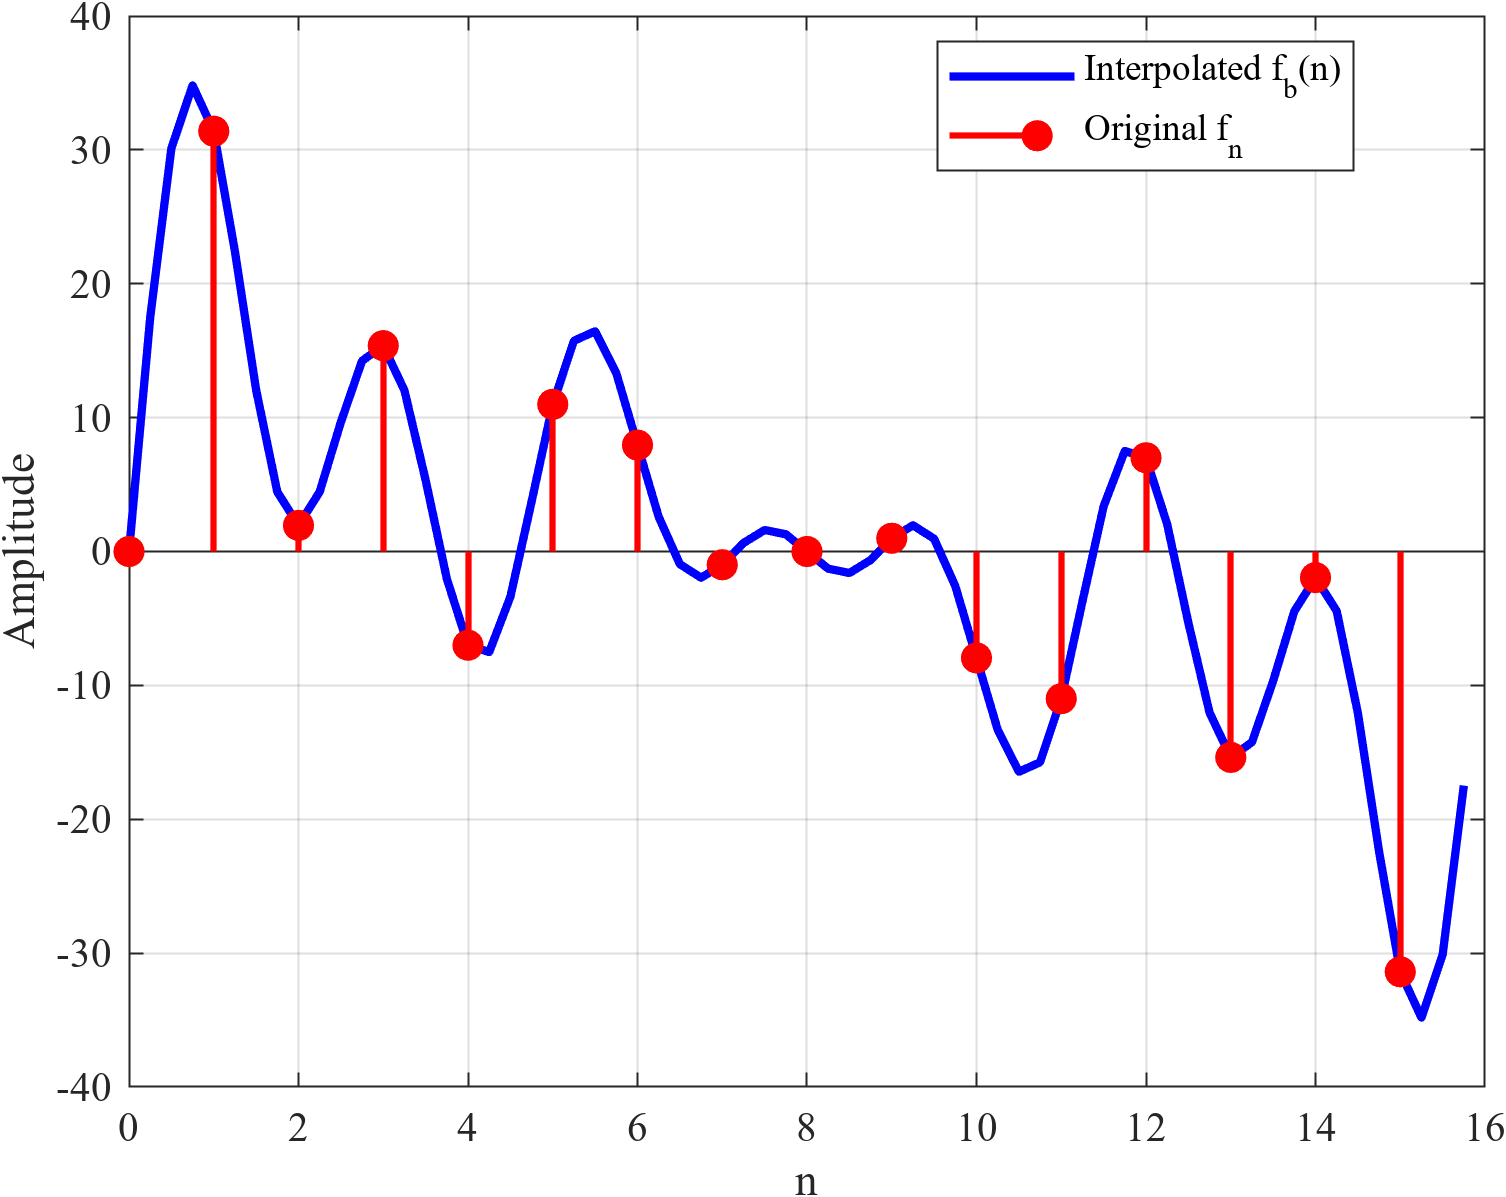
\includegraphics[width=0.8\textwidth]{f_b.png}
    \caption{Comparison of Interpolated Signal with Original Samples}
\end{figure}

Again, I had to do some scaling to preserve the total energy of the plot (See the $\times 4$ in the definition of $F_b$). Other than that, we can see the "identical-ity" of the two. $f_b(n)$ has more granularity than $f(n)$. 


\newpage
\section*{II. Signal Scrambling}
The objective of this exercise is to implement a simple digital speech scrambler.

We use the microphone of of our computer to record a short speech signal $g(t)$, and digitize the speech signal with the A/D tool in Audacity into the discrete form $g(n)$.

\begin{lstlisting}[language=Octave, caption=Reading in Audio File]
[g_n, f_s] = audioread('g_n.wav');
\end{lstlisting}


\subsection*{1. DFT Spectrum}
The DFT spectrum $G(k)$ of the digitized speech signal $g(n)$ is shown below:

\begin{lstlisting}[language=Octave, caption=FFT of Audio Sequence]
G_k = fft(g_n);
G_k_shifted = fftshift(G_k);
\end{lstlisting}

\begin{figure}[H]
    \centering
    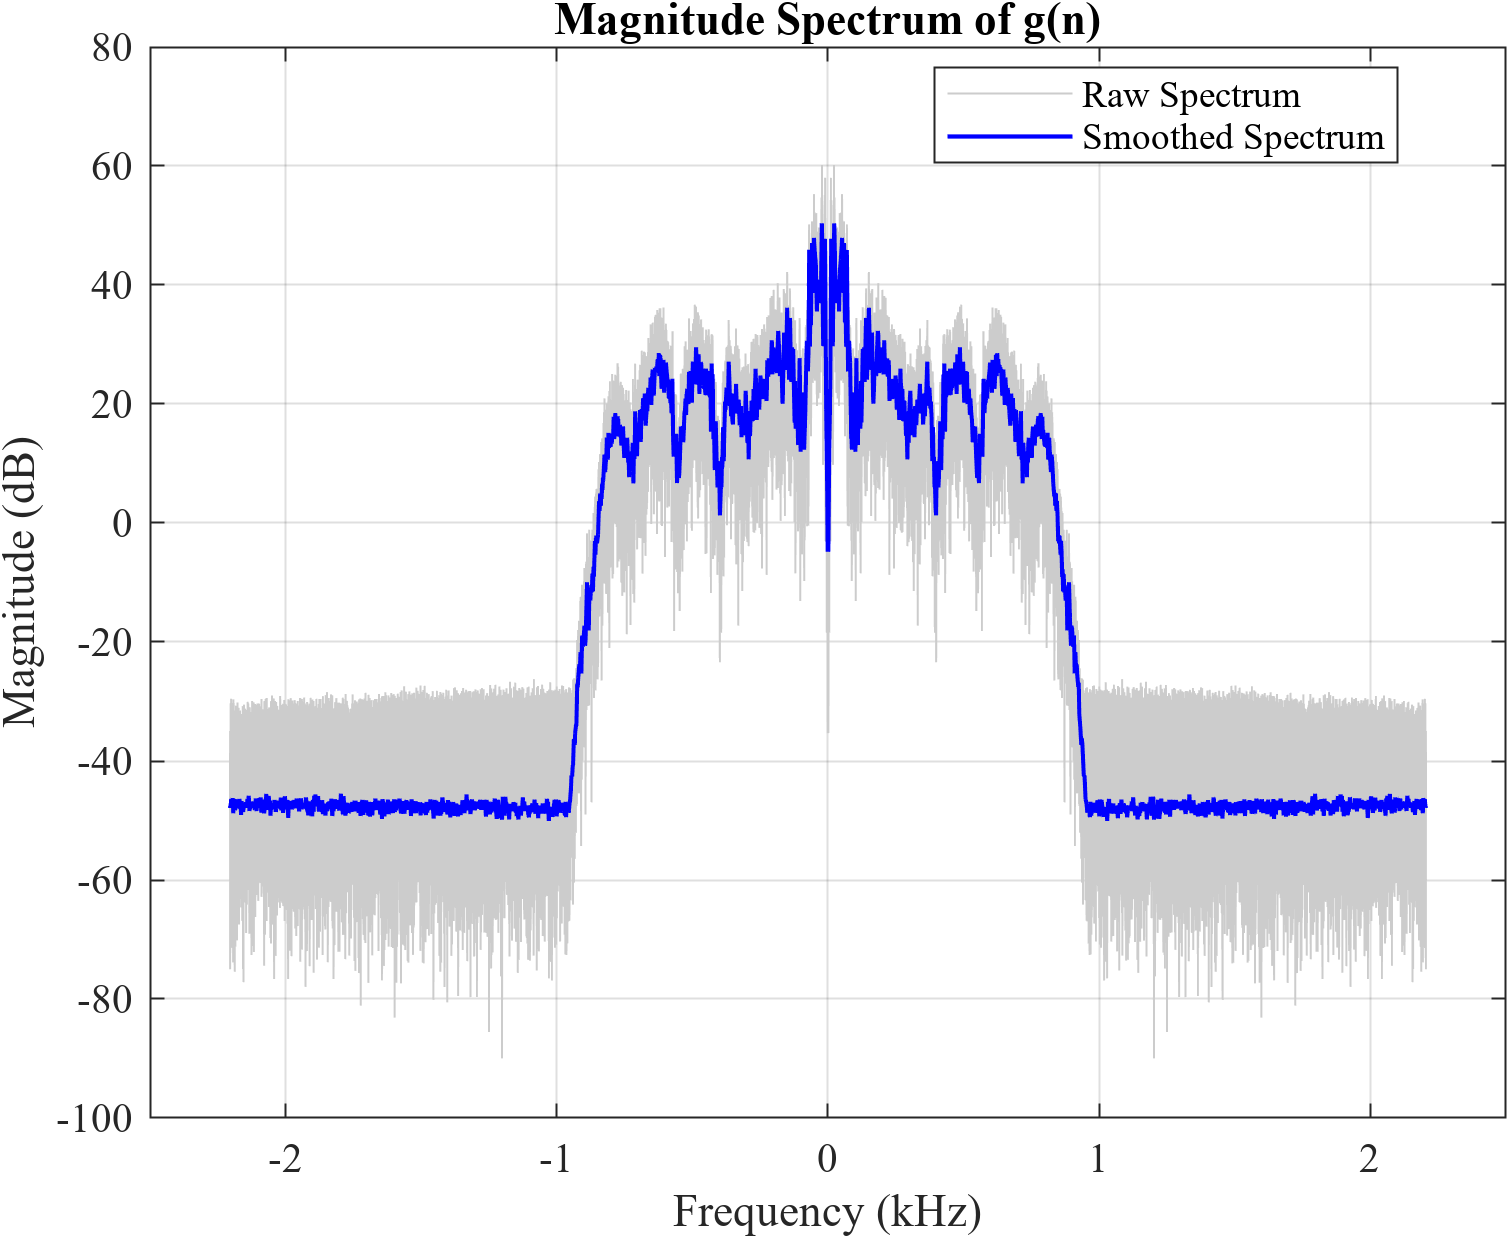
\includegraphics[width=0.8\textwidth]{G_k.png}
    \caption{Magnitude Spectrum of Original Speech Signal}
\end{figure}


\newpage
\subsection*{2. Speech Scrambling}
The speech signal is scrambled by multiplying it with an alternating sequence of +1 and -1. 

\begin{lstlisting}[language=Octave, caption=FFT of Hilbert Sequence]
scrambling_seq = ones(size(g_n));
scrambling_seq(2:2:end) = -1;

g_hat_n = g_n .* scrambling_seq;
audiowrite('g_hat_n.wav', g_hat_n, f_s);

G_hat_k = fft(g_hat_n);
G_hat_k_shifted = fftshift(G_hat_k);
\end{lstlisting}

\begin{figure}[H]
    \centering
    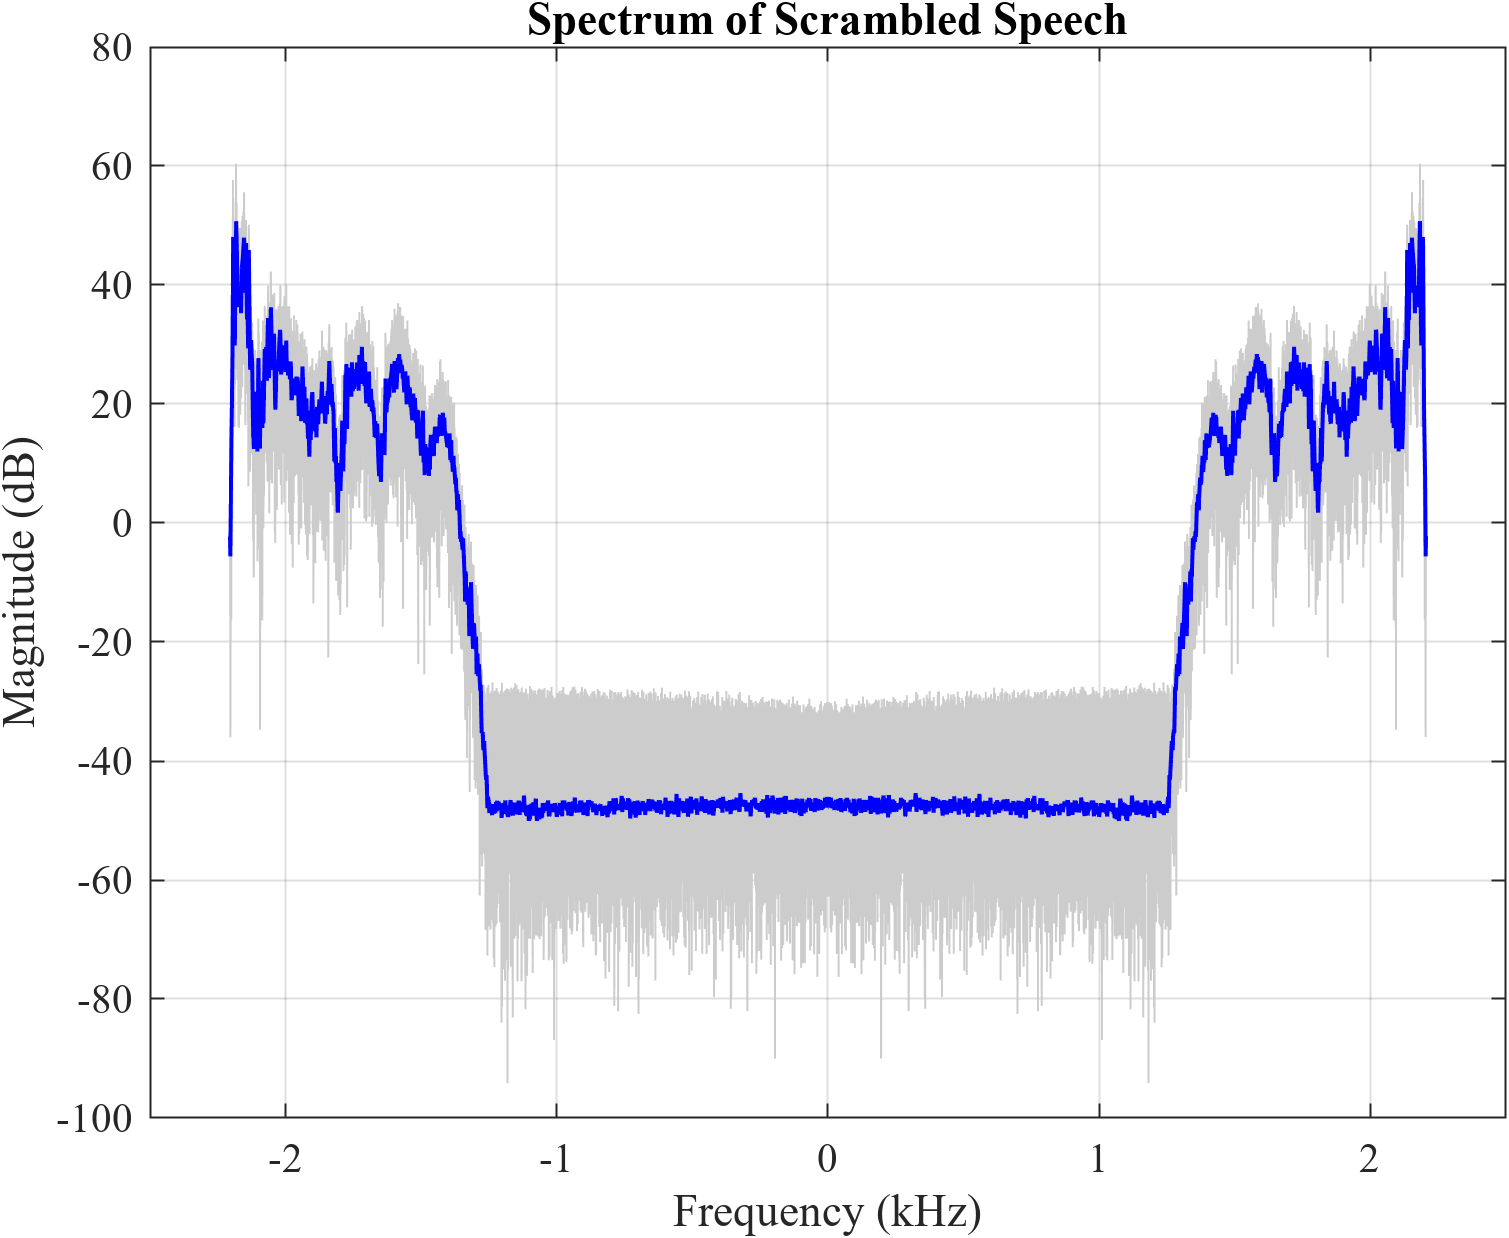
\includegraphics[width=0.8\textwidth]{G_hat_k.png}
    \caption{Spectrum of Scrambled Speech}
\end{figure}

The scrambled audio $\hat{g}_n$ is completely unintelligible. It sounds like the high pitched squealing of an adult in a cartoon. Or the feverish screeches of a pulley that needs greasing. The speech is thouroughly "scrambled".


\newpage
\subsection*{3. Descrambling}
The descrambling process uses the same alternating sequence. When there is a synchronization offset, it results in -g(t) instead of g(t).

\begin{lstlisting}[language=Octave, caption=Descrambling]
descrambled_g_n = g_hat_n .* scrambling_seq;

audiowrite('descrambled_g_n.wav', descrambled_g_n, f_s);
\end{lstlisting}

The descrambled audio is completely intelligible. It seems no different at all from the original audio, qualitatively or quantitatively. I pulled up the graphs of each and the descrambled signal is not actually inverted. I did so myself by multiplying the whole thing by $-1$ and listened to thaat, which again, sounded exactly the same.

\newpage
\section*{III. Hilbert Transform}

\subsection*{1. Periodic Signal f(t)}
The Hilbert transform of the periodic signal $f(t)$ is computed and compared with the original signal:

\begin{figure}[H]
    \centering
    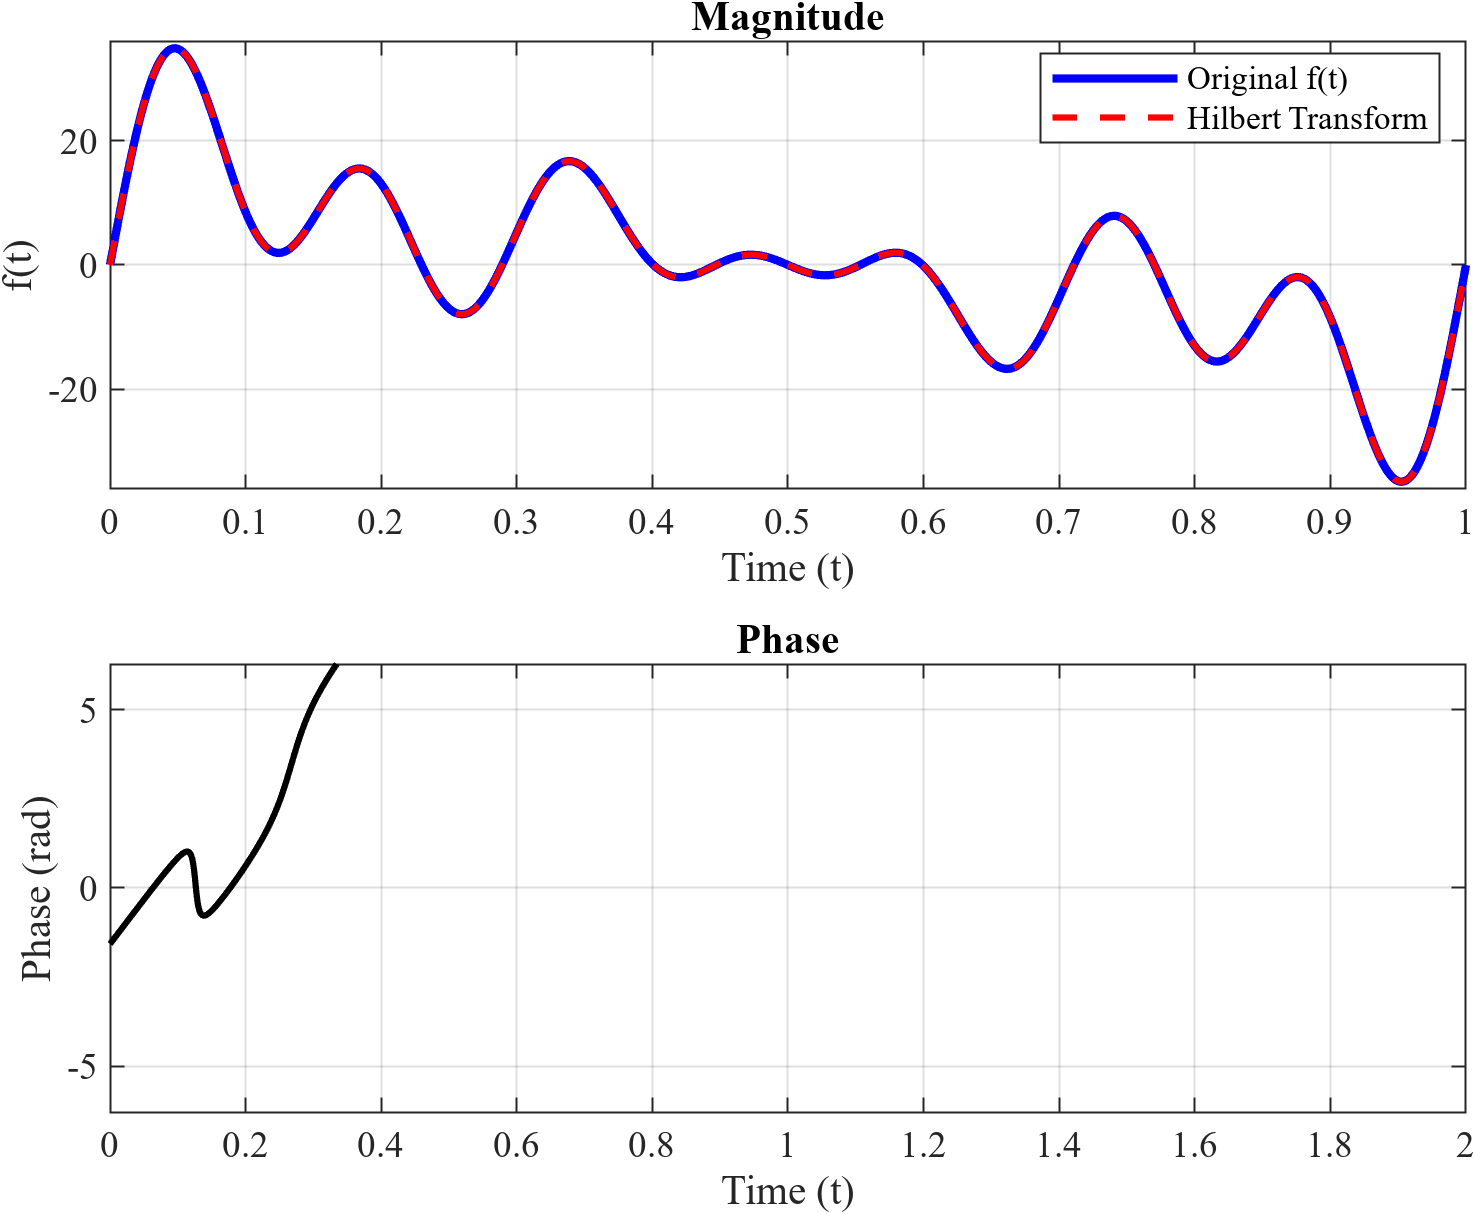
\includegraphics[width=0.8\textwidth]{f_t.png}
    \caption{Original Signal and its Hilbert Transform}
\end{figure}

The real part of the two signals is identical, as expected.
The imaginary parts, however differ greatly. $f(t)$ being an entirely real signal is constantly $0$, but the imaginary part of $\mathcal{H}\{f(t)\}$ is periodic with respect to $t$ correleted and sometimes inversely correlated to the real part.


\newpage
\subsection*{2. Speech Signal g(t)}
The Hilbert transform is applied to the speech signal g(t), and the result is saved as an audio file for audible comparison.

\begin{lstlisting}[language=Octave, caption=Hilbert Transform of $g(n)$]
hilbert_g_n = hilbert(g_n);

audiowrite('hilbert_g_n.wav', real(hilbert_g_n), f_s);
\end{lstlisting}

The audio is completely intelligible. In fact, it is the exact same becuase I had to use only the real part of the signal before MATLAB would let me call \lstinline[language=Octave]|audiowrite(.)|.

\newpage
\section*{Summary}
\begin{itemize}
    \item Demonstrated DFT-based interpolation in both frequency and time domains, showing how zero-padding increases resolution.
    \item Implemented and analyzed a simple speech scrambling technique using multiplication by an alternating sequence.
    \item Verified that descrambling restores the original speech, confirming the reversibility of the scrambling process.
    \item Explored the Hilbert transform for both periodic and speech signals, observing effects on real and imaginary components.
\end{itemize}
\end{document}